\documentclass{beamer}

\mode<presentation> 
{
	\usetheme{Madrid}
}

\usepackage{graphicx, graphics}
\usepackage{booktabs}
\usepackage{multicol}
\usepackage{apacite}
\setlength{\columnseprule}{0.4pt}
\usepackage{tcolorbox}
\DeclareGraphicsExtensions{.pdf,.png,.jpg,.gif}

\title{FID Data Reconstruction}
\author[Jaewoong Lee]{20161206 JaewoongLee}
\institute[UNIST]
{
	Ulsan National Institute of Science and Technology
	\medskip
	\newline
	\textit{jwlee230@unist.ac.kr}
}
\date{\today}

\begin{document}
	\begin{frame}
		\titlepage
	\end{frame}

	\begin{frame}
		\frametitle{Overview}
		\tableofcontents
	\end{frame}

	\section{Theory}
	\begin{frame}
		\frametitle{Brain Development}
		\begin{itemize}
			\item Brain development is protract process that begins in the 3rd gestational week, and it continues for an extended period post-natally. \cite{ref:brain1}
			\item MRI studies of structural and functional changes in the developing human brain. \cite{ref:brain2}
		\end{itemize}
	\end{frame}

	\begin{frame}
		\frametitle{Substantia Nigra (SN)}
		\begin{itemize}
			\item SN is an anatomically heterogeneous nucleus with regional alternation in striatal projections and distribution of histo-chemical markers. \cite{ref:nigra1}
			\item Dopamine contributes to the processing of signals in SN. \cite{ref:nigra3}
			\item Dopaminergic neurons have been developed in SN. \cite{ref:nigra4}
		\end{itemize}
	\end{frame}

	\begin{frame}
		\frametitle{Corpus callosum (CC)}
		\begin{itemize}
			\item CC is a wid and thick nerve tract, beneath the cerebra cortex in the brain. 
			\item CC plays an major role in inter-hemispheric integration and communication. \cite{ref:cc1}
			\item The size of CC differs upon disease, occupations, genders, and etc. 
			\item Growth of CC was noticed from the 4th fetal month to maturity. \cite{ref:cc5, ref:cc6}
		\end{itemize}
	\end{frame}

	\begin{frame}
		\frametitle{Development in Rats and Humans}
		\begin{itemize}
			\item Some papers made approximate one-to-one correspond between development of rats and humans. \cite{ref:dev2}
			\item The relation between rats and human aging:
			\begin{itemize}
				\item 6 week in Rat = 4.5 years in Human
				\item 4 month in Rat = 12 years in Human
				\item 20 month in Rat = 50 years in Human
			\end{itemize}
		\end{itemize}
	\end{frame}
	
	\section{Result}
	\begin{frame}
		\frametitle{RARE-VTR FID Image}
		\begin{figure}
			$\begin{array}{ccc}
				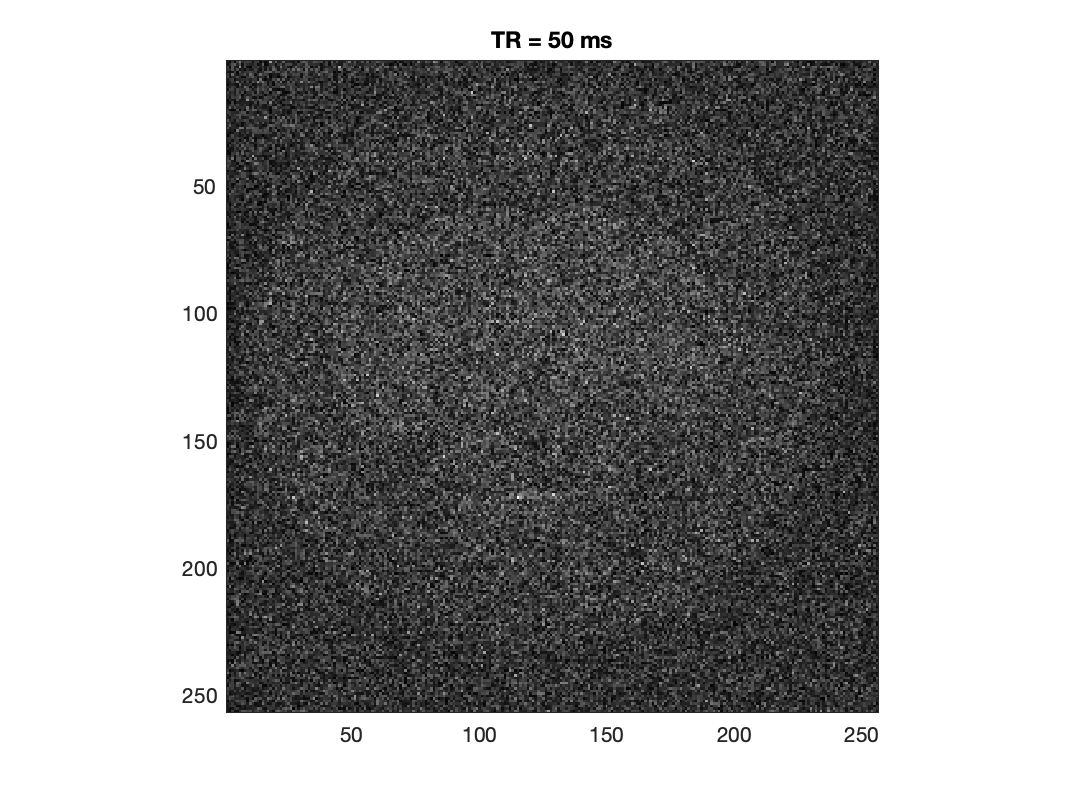
\includegraphics[width=0.3 \linewidth]{figures/VTR_6week/vtr_6week_1.png}
				&
				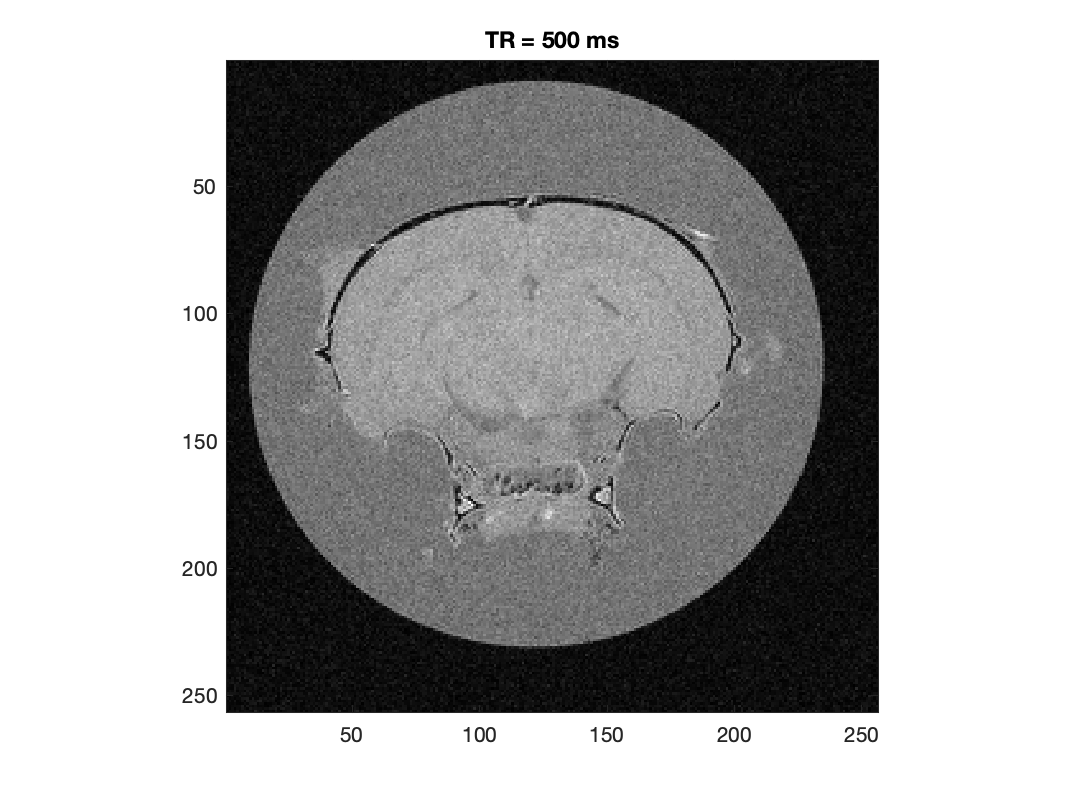
\includegraphics[width=0.3 \linewidth]{figures/VTR_6week/vtr_6week_5.png}
				&
				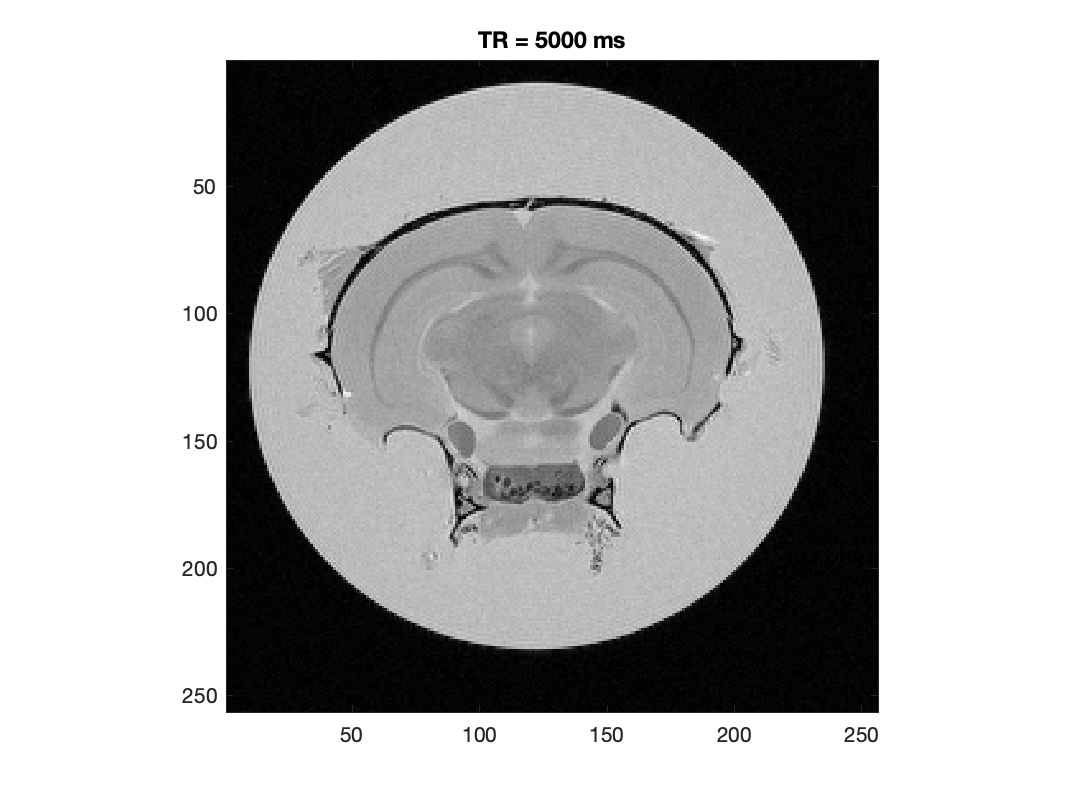
\includegraphics[width=0.3 \linewidth]{figures/VTR_6week/vtr_6week_10.png}
				\\
			\end{array}$
			\caption{RARE-VTR FID Images in 6 week}
		\end{figure}
	\end{frame}

	\begin{frame}
		\frametitle{MSME FID Image}
		\begin{figure}
			$\begin{array}{ccc}
				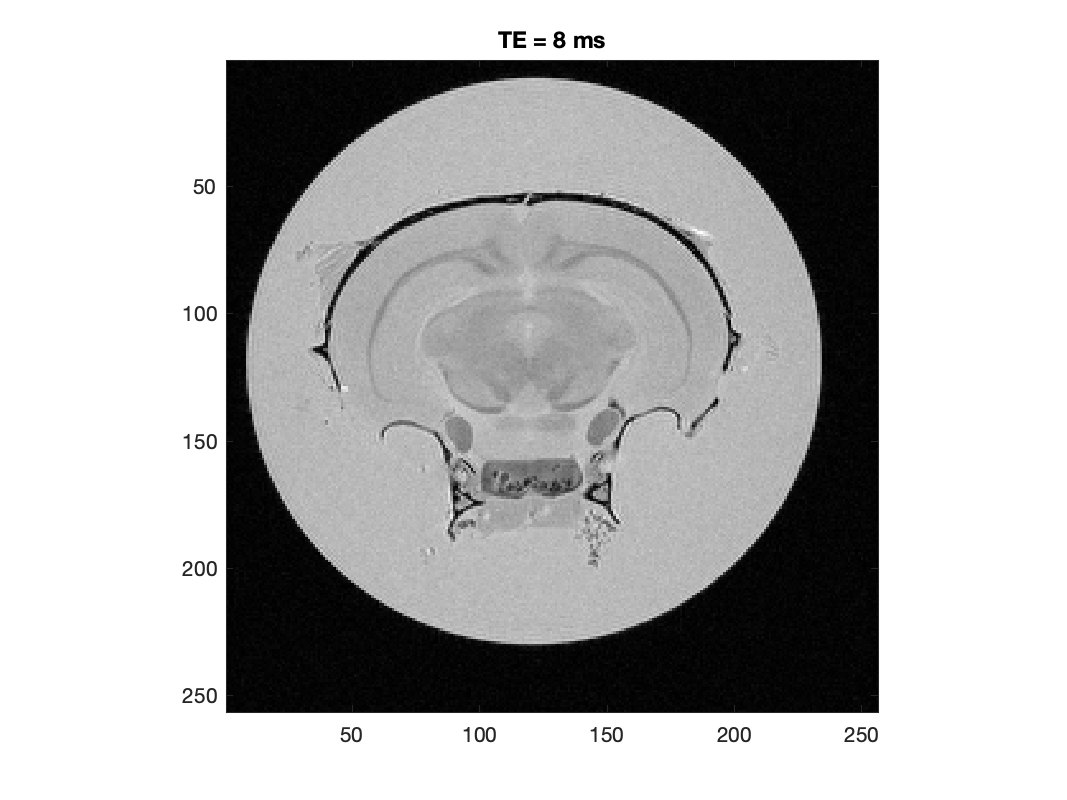
\includegraphics[width=0.3 \linewidth]{figures/MSME_6week/msme_6week_1.png}
				&
				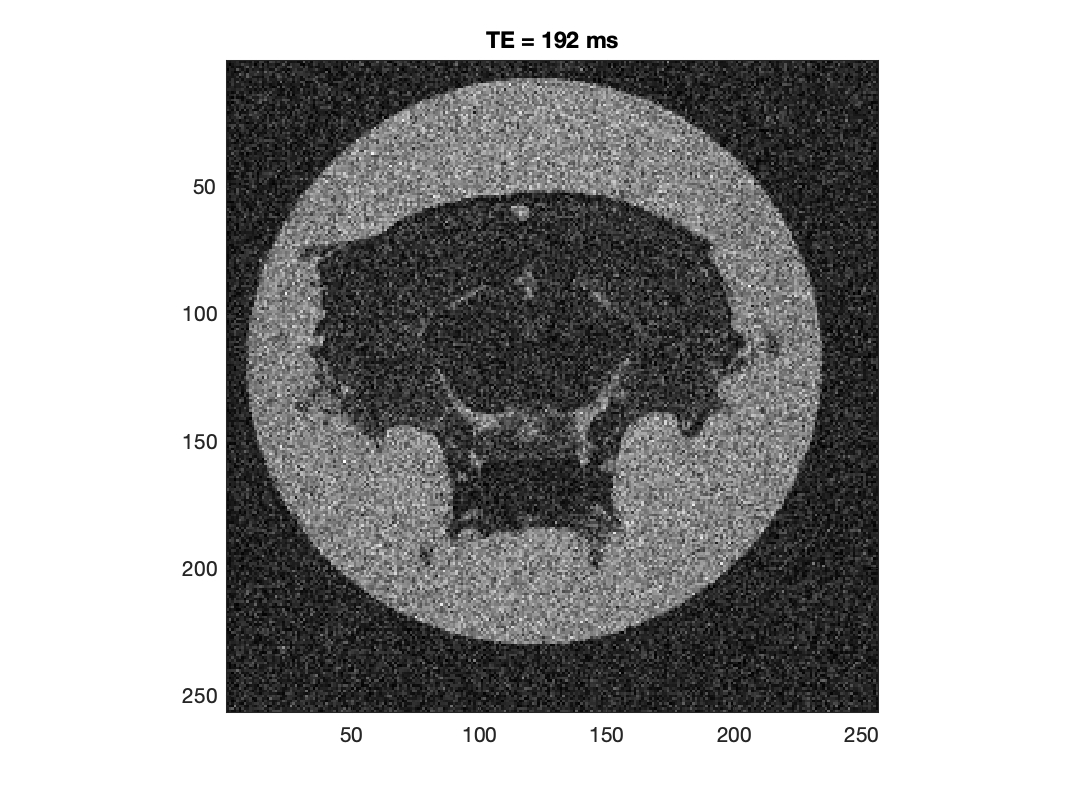
\includegraphics[width=0.3 \linewidth]{figures/MSME_6week/msme_6week_24.png}
				&
				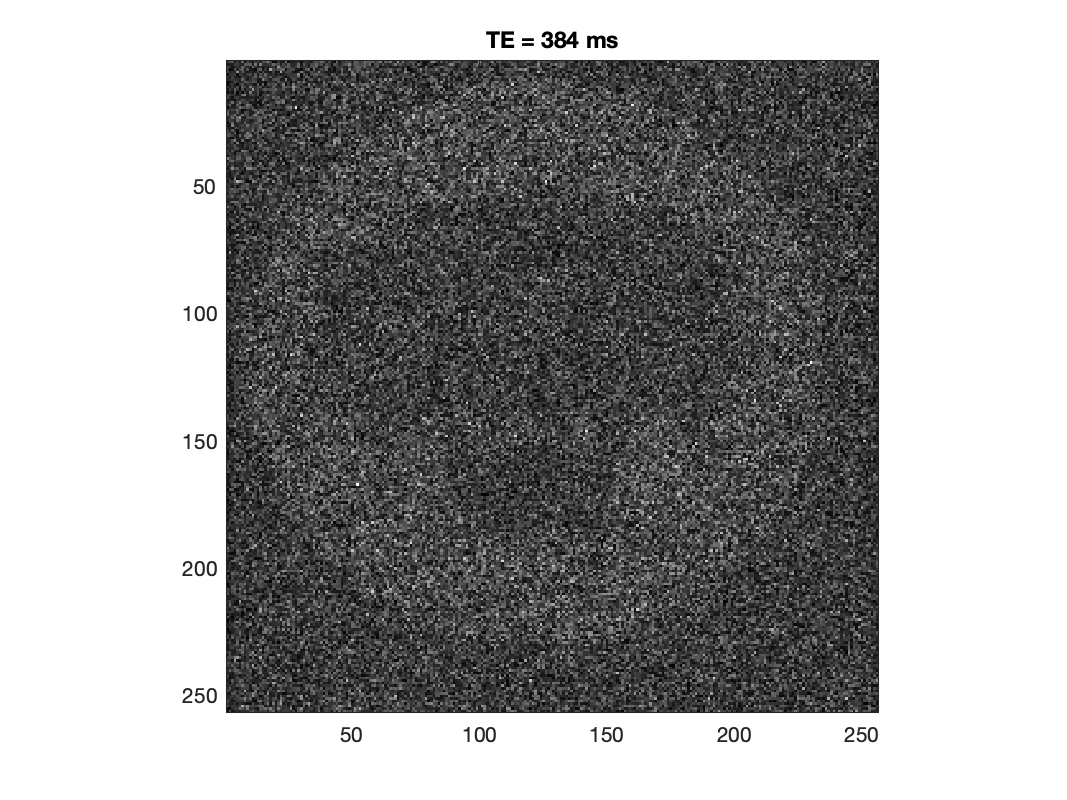
\includegraphics[width=0.3 \linewidth]{figures/MSME_6week/msme_6week_48.png}
				\\
			\end{array}$
			\caption{MSME FID Images in 6 week}
		\end{figure}
	\end{frame}

	\begin{frame}
		\frametitle{MGE FID Image}
		\begin{figure}
			$\begin{array}{ccc}
				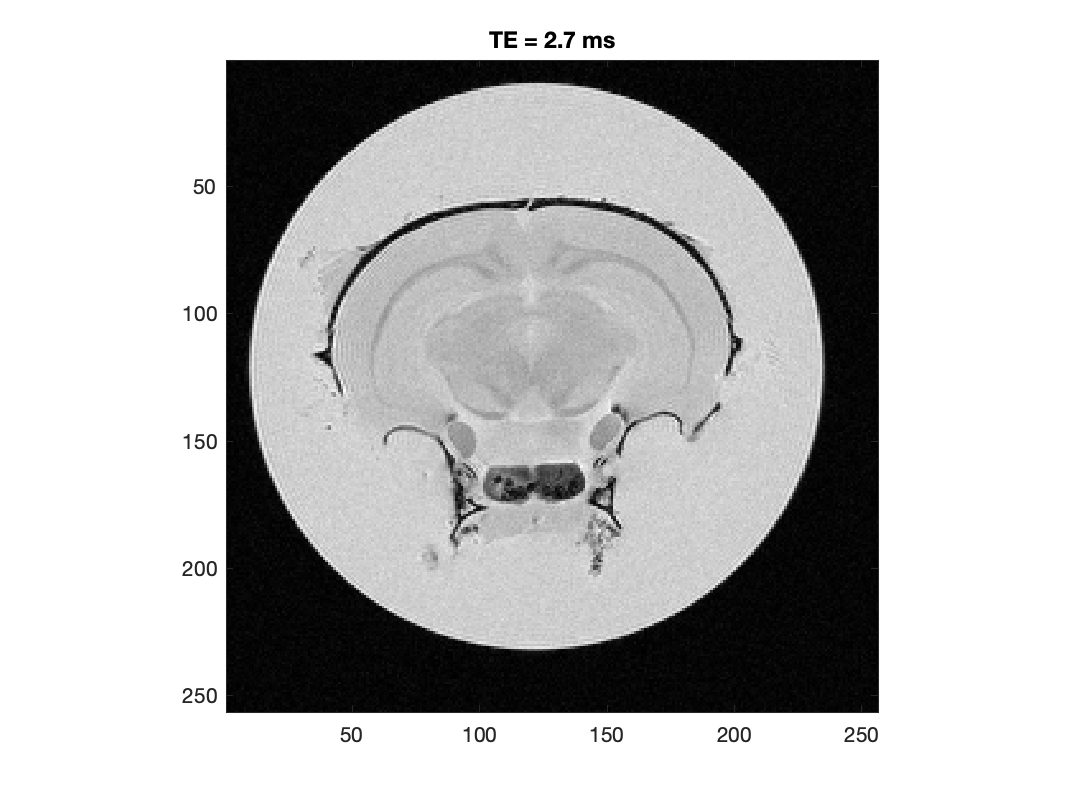
\includegraphics[width=0.3 \linewidth]{figures/MGE_6week/mge_6week_1.png}
				&
				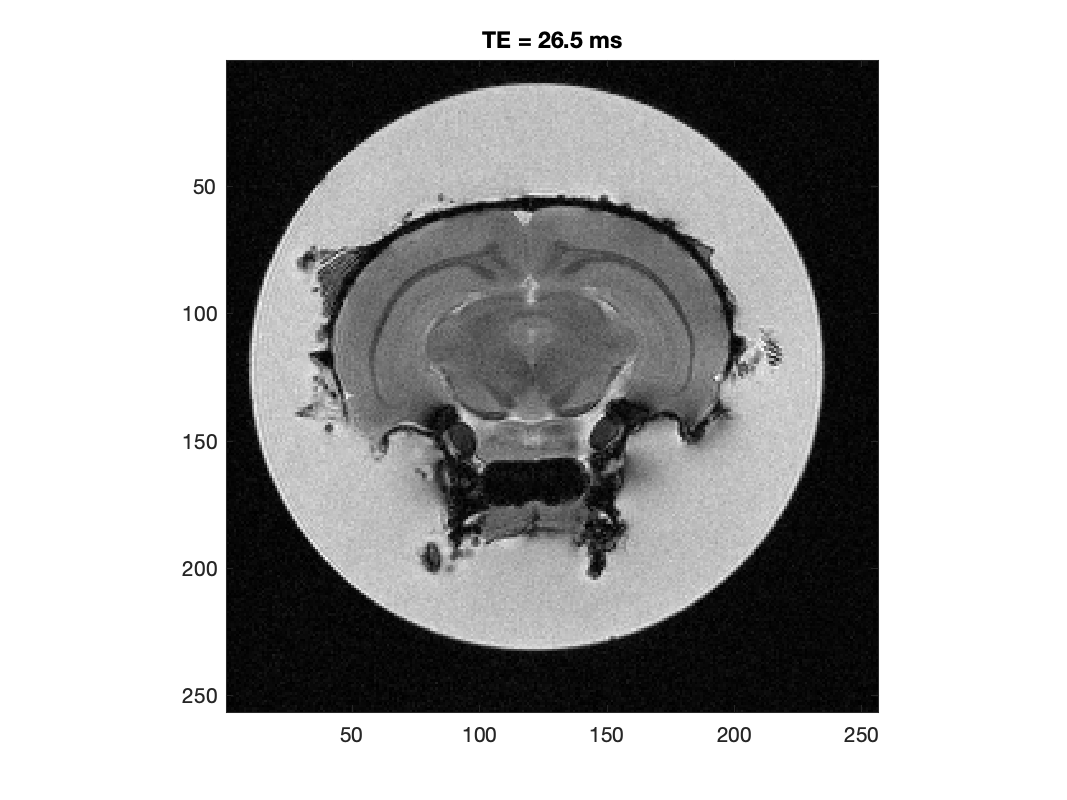
\includegraphics[width=0.3 \linewidth]{figures/MGE_6week/mge_6week_8.png}
				&
				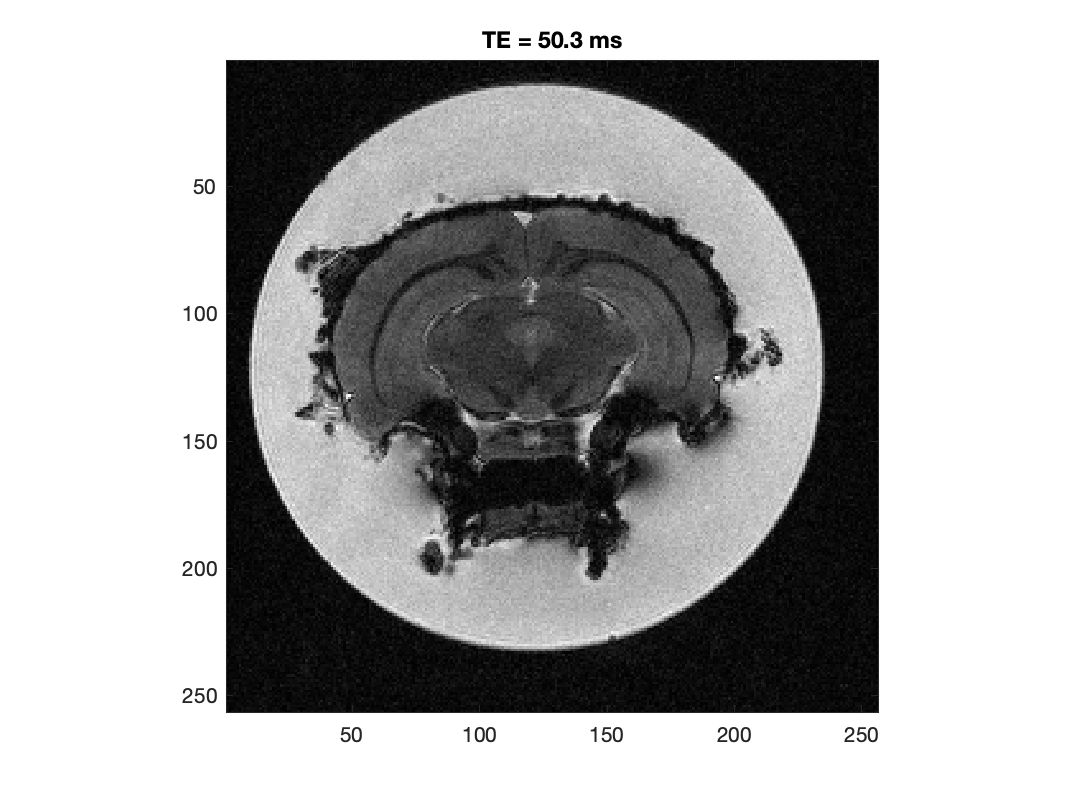
\includegraphics[width=0.3 \linewidth]{figures/MGE_6week/mge_6week_15.png}
				\\
				\end{array}$
			\caption{MGE FID Images in 6 week}
		\end{figure}
	\end{frame}

	\begin{frame}
		\frametitle{$T_1$ Fitting}
		\begin{figure}
			$\begin{array}{ccc}
			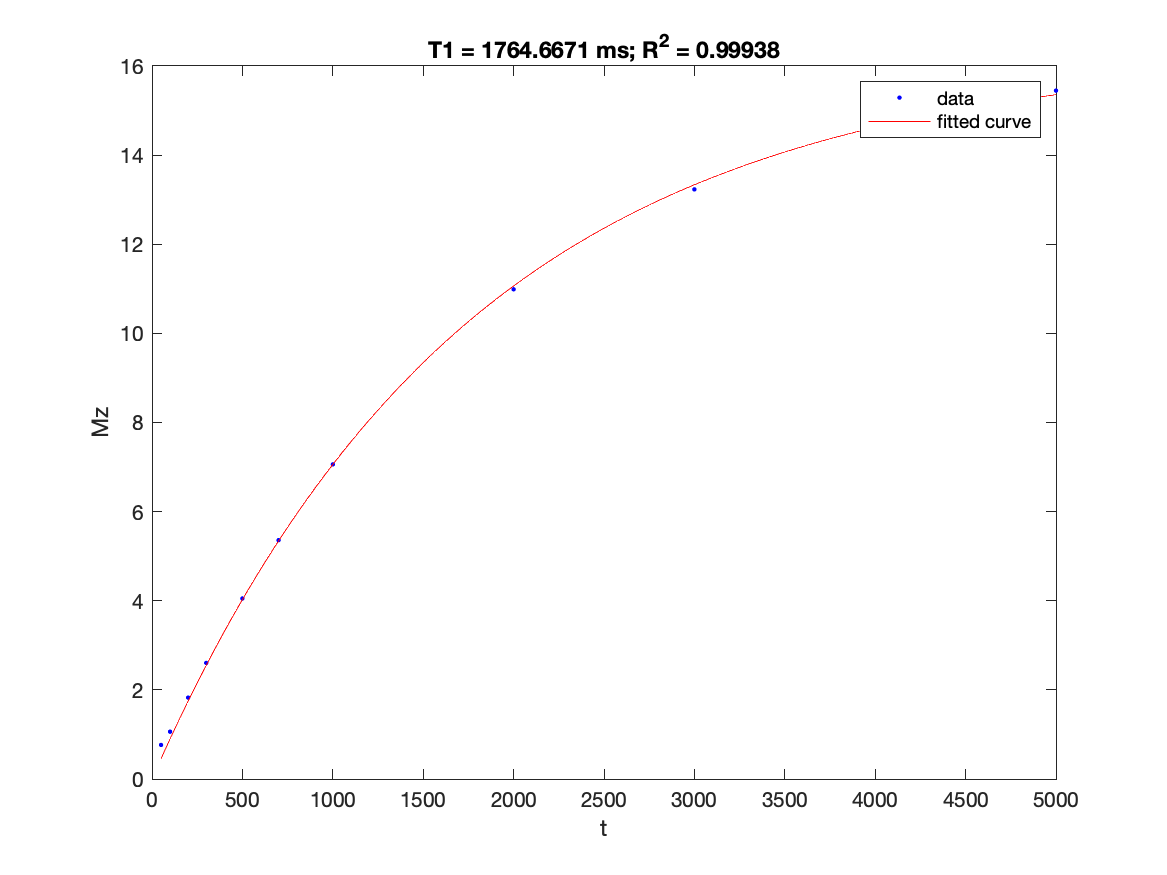
\includegraphics[width=0.3 \linewidth]{figures/T1_fit/T1_6week_fit.png}
			&
			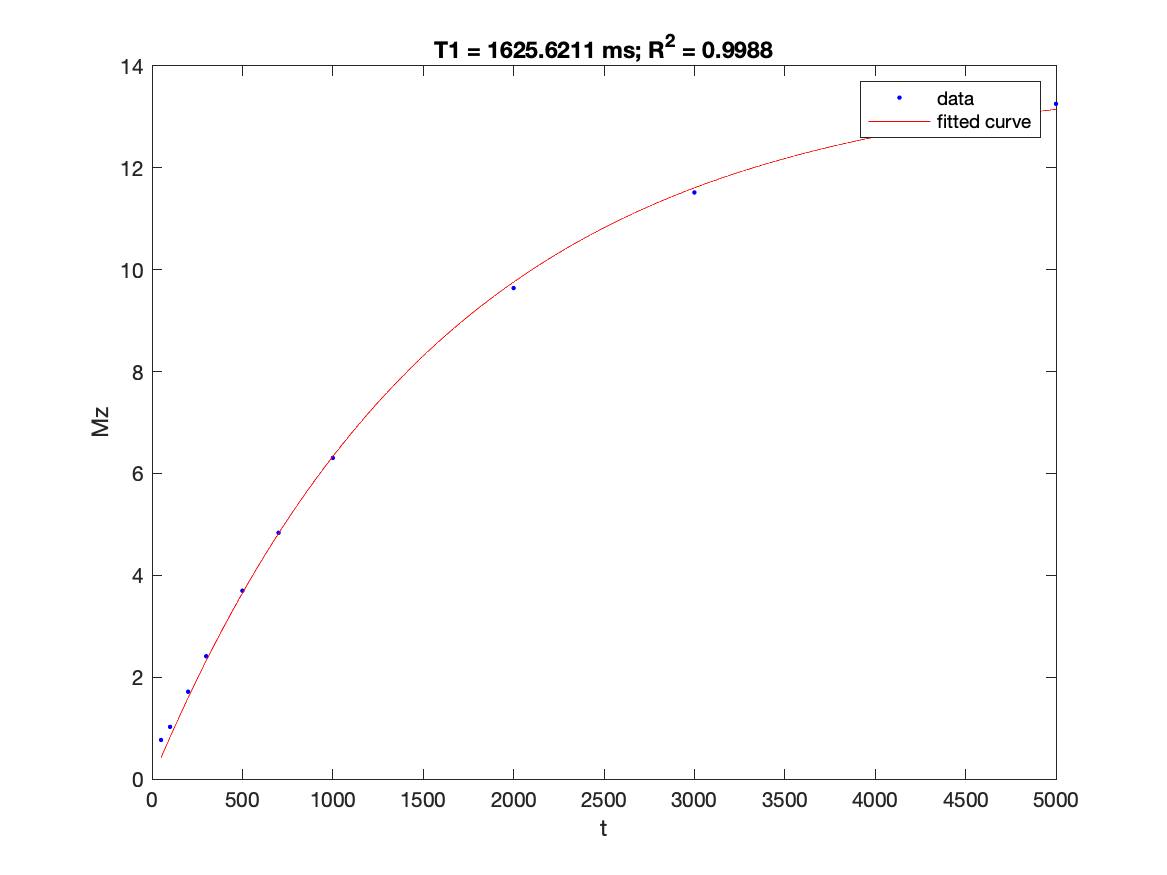
\includegraphics[width=0.3 \linewidth]{figures/T1_fit/T1_4month_fit.png}
			&
			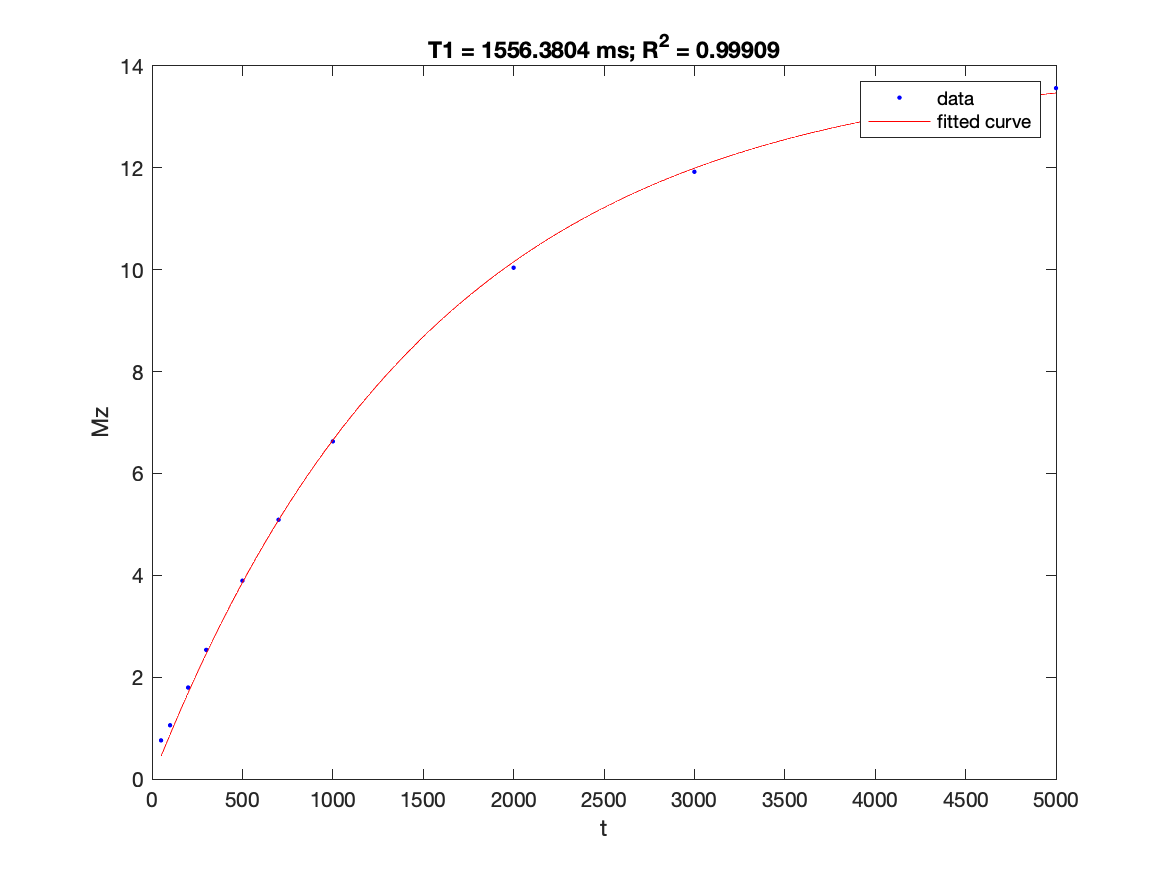
\includegraphics[width=0.3 \linewidth]{figures/T1_fit/T1_20month_fit.png}
			\\
			\end{array}$
			\caption{$T_1$ Fitting}
		\end{figure}
	\end{frame}

	\begin{frame}
		\frametitle{$T_2$ Fitting}
		\begin{figure}
			$\begin{array}{ccc}
			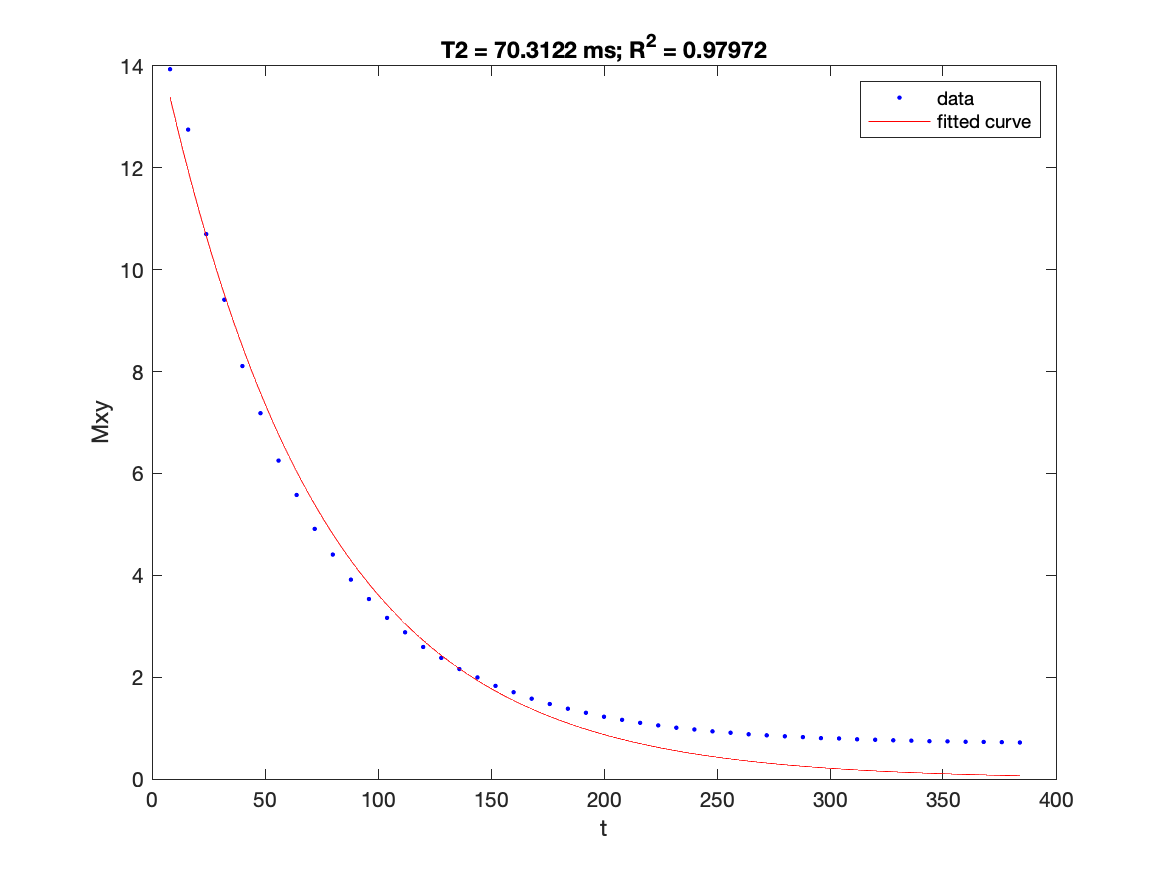
\includegraphics[width=0.3 \linewidth]{figures/T2_fit/T2_6week_fit.png}
			&
			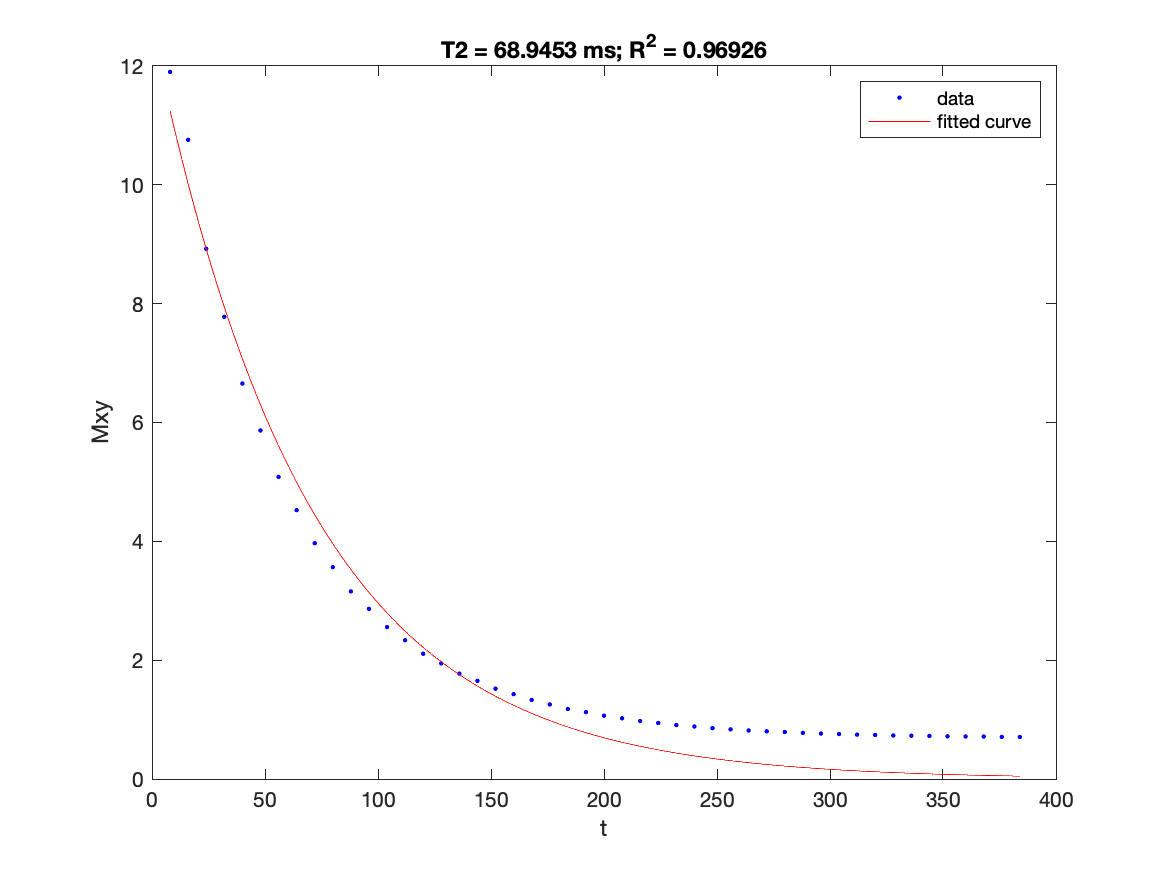
\includegraphics[width=0.3 \linewidth]{figures/T2_fit/T2_4month_fit.png}
			&
			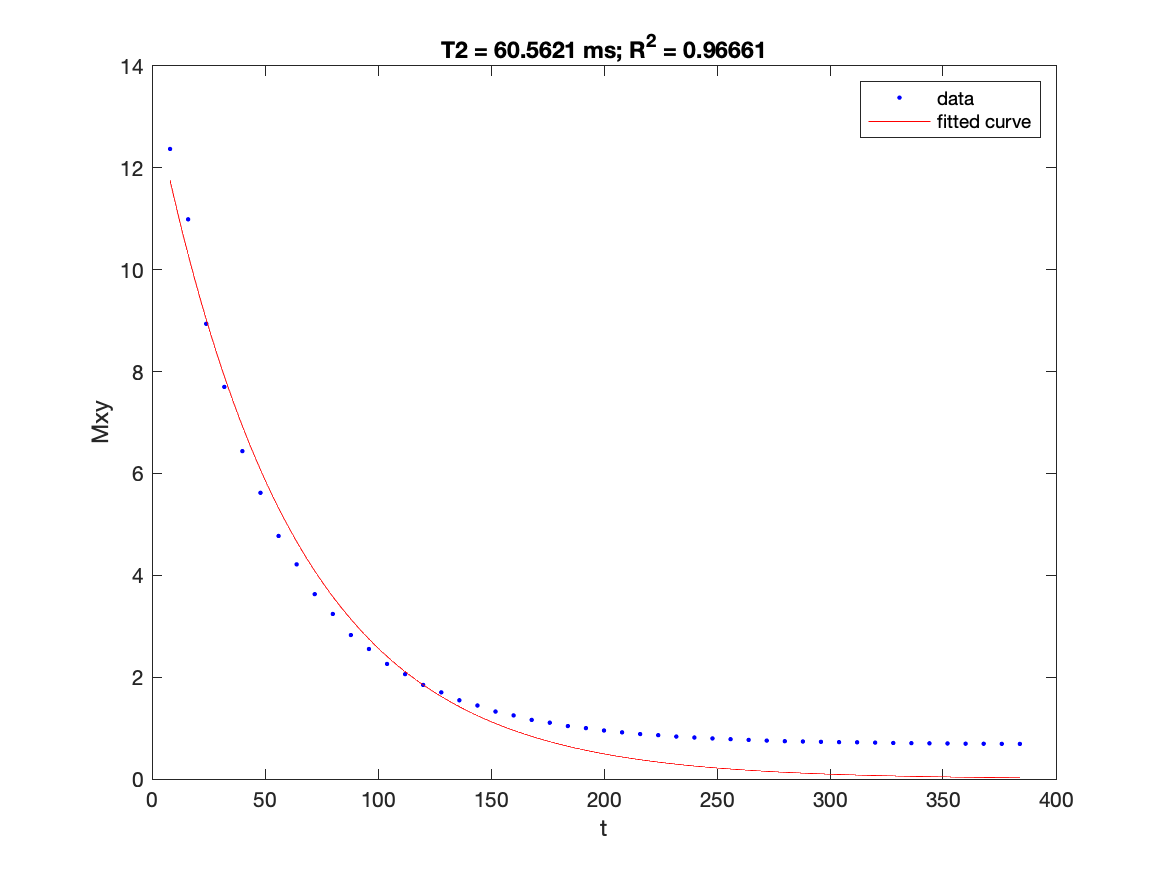
\includegraphics[width=0.3 \linewidth]{figures/T2_fit/T2_20month_fit.png}
			\\
			\end{array}$
			\caption{$T_2$ Fitting}
		\end{figure}
	\end{frame}

	\begin{frame}
		\frametitle{$T_2^*$ Fitting}
		\begin{figure}
			$\begin{array}{ccc}
			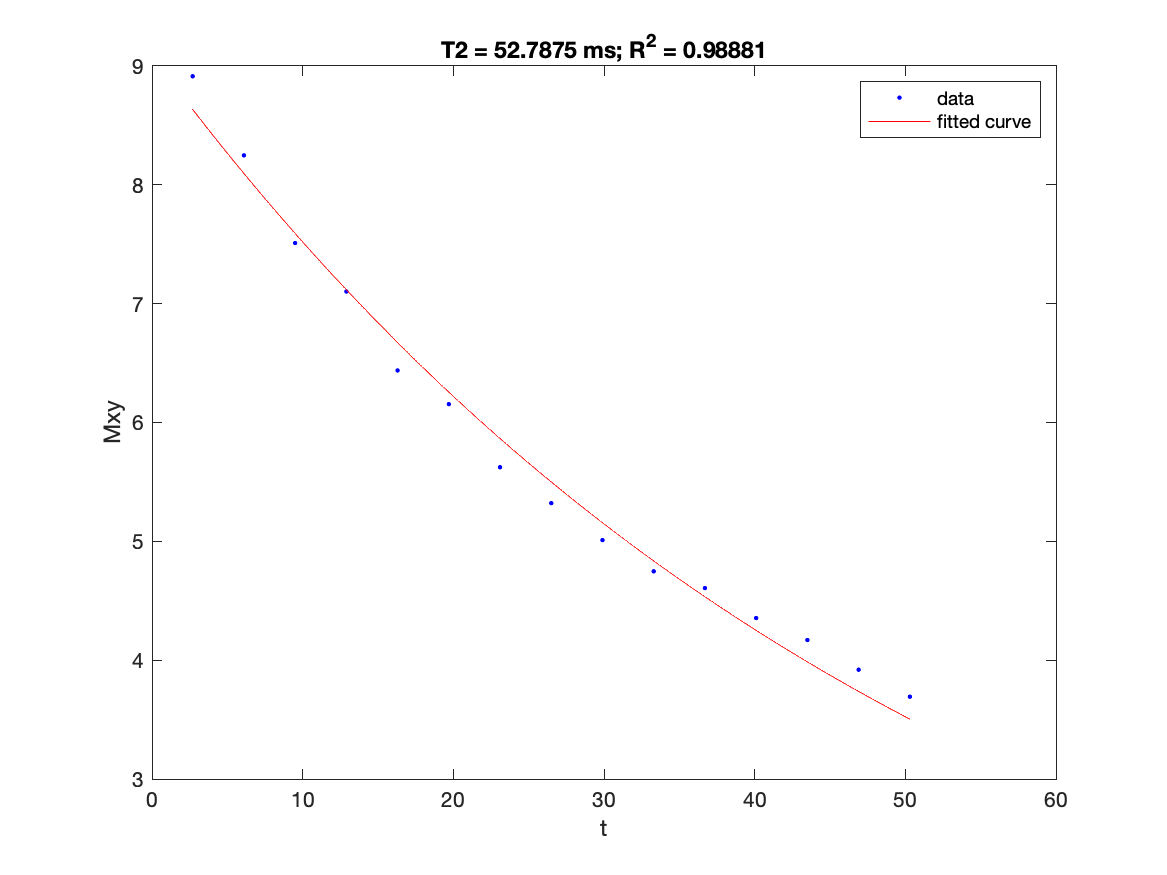
\includegraphics[width=0.3 \linewidth]{figures/T2star_fit/T2star_6week_fit.png}
			&
			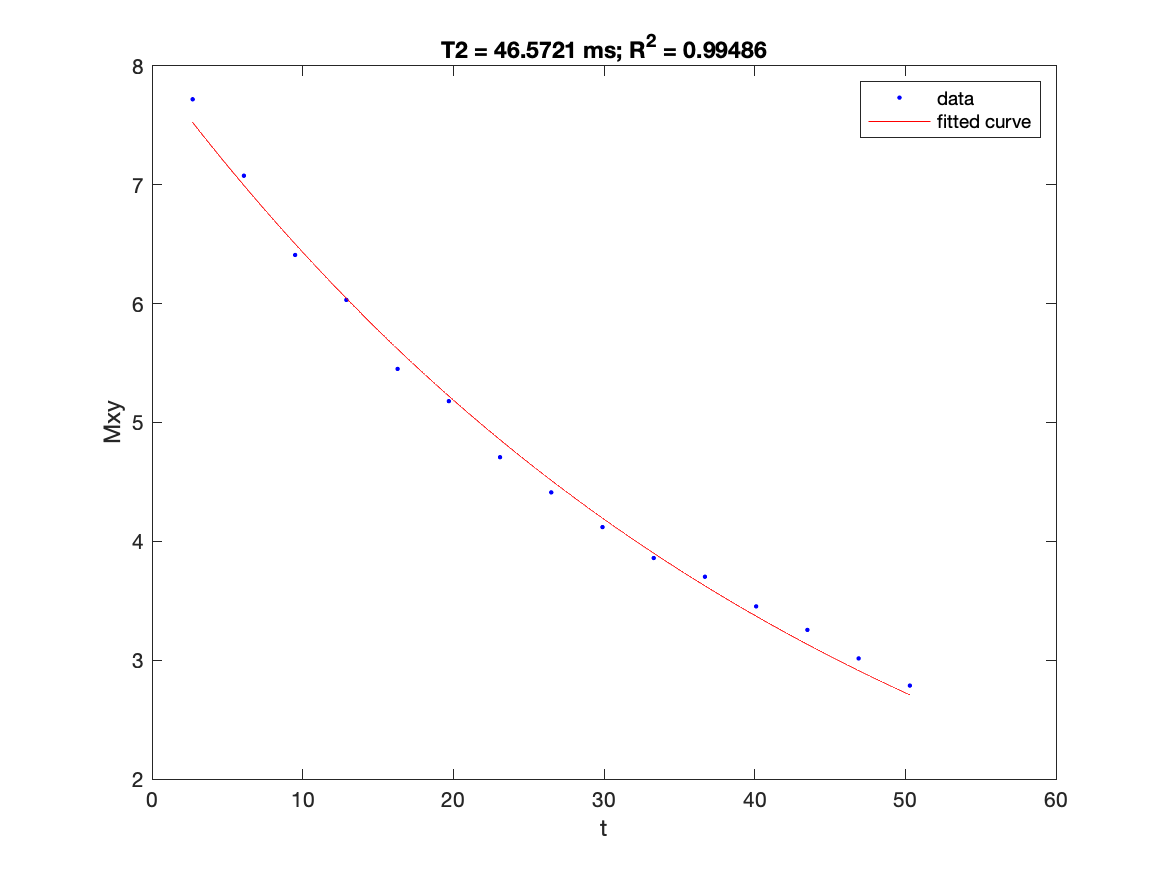
\includegraphics[width=0.3 \linewidth]{figures/T2star_fit/T2star_4month_fit.png}
			&
			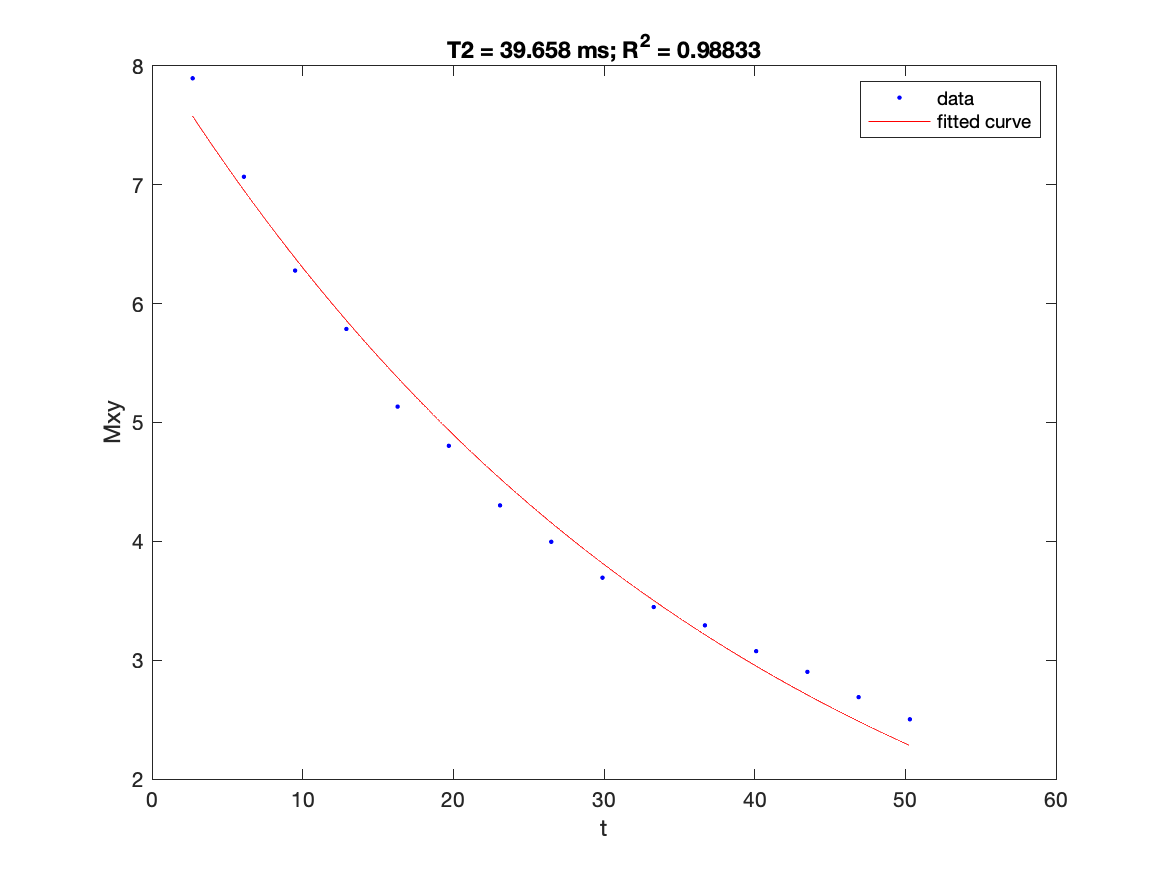
\includegraphics[width=0.3 \linewidth]{figures/T2star_fit/T2star_20month_fit.png}
			\\
			\end{array}$
			\caption{$T_2^*$ Fitting}
		\end{figure}
	\end{frame}

	\begin{frame}
		\frametitle{$T_1$ Mapping}
		\begin{figure}
			$\begin{array}{ccc}
				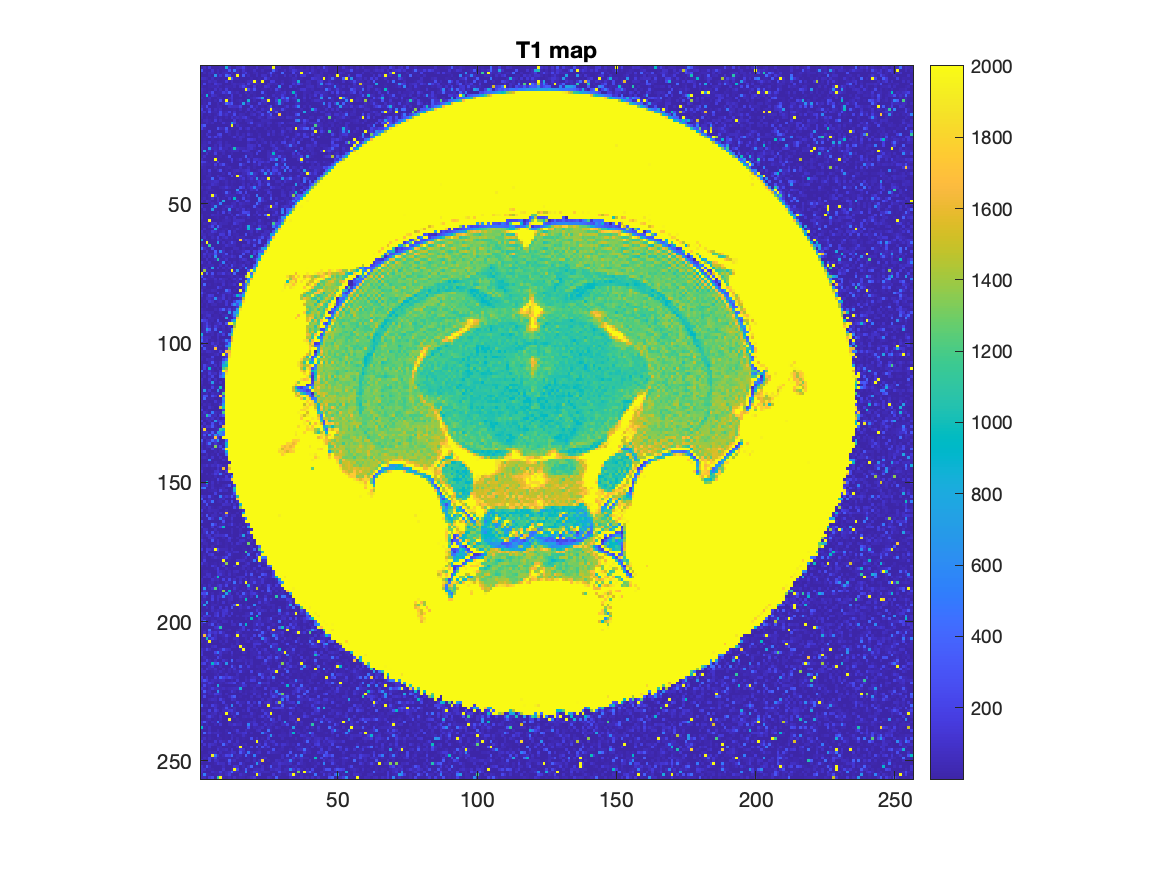
\includegraphics[width=0.3 \linewidth]{figures/T1_map/T1_6week_map.png}
				&
				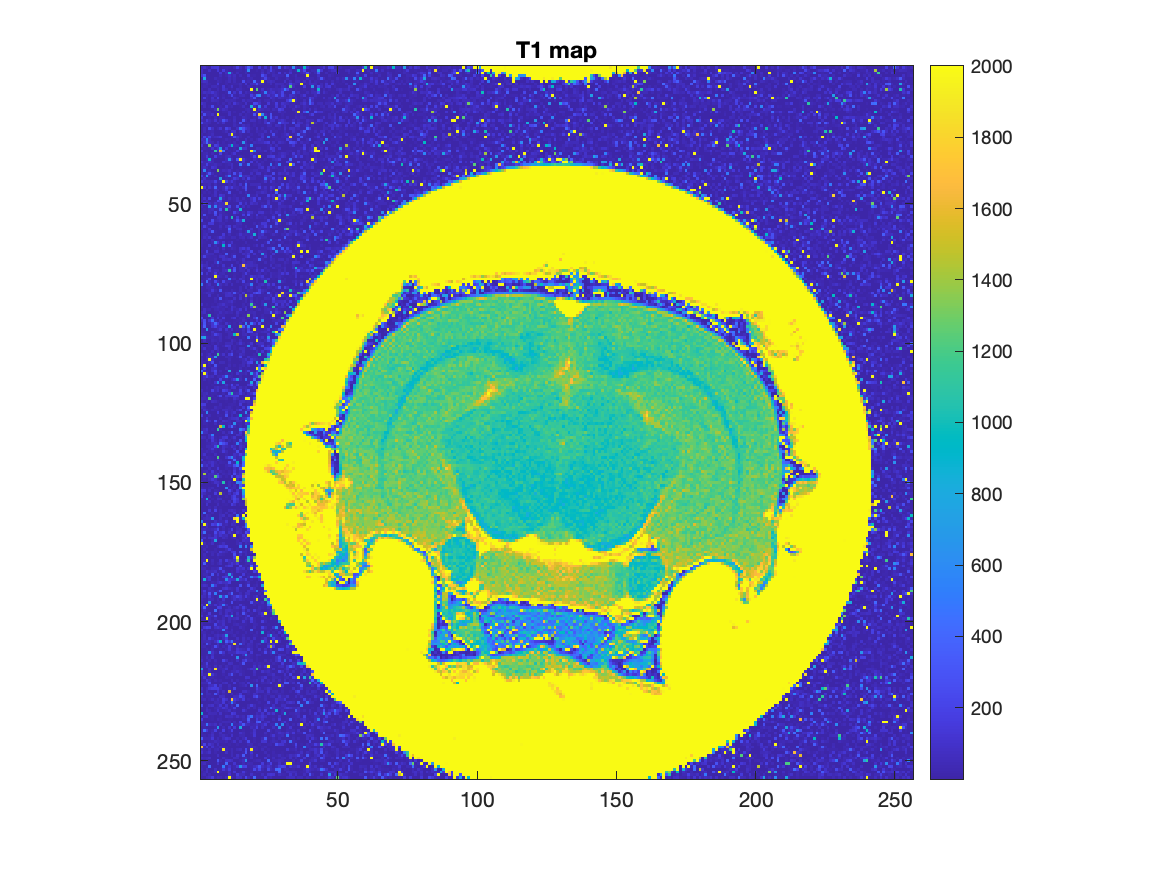
\includegraphics[width=0.3 \linewidth]{figures/T1_map/T1_4month_map.png}
				&
				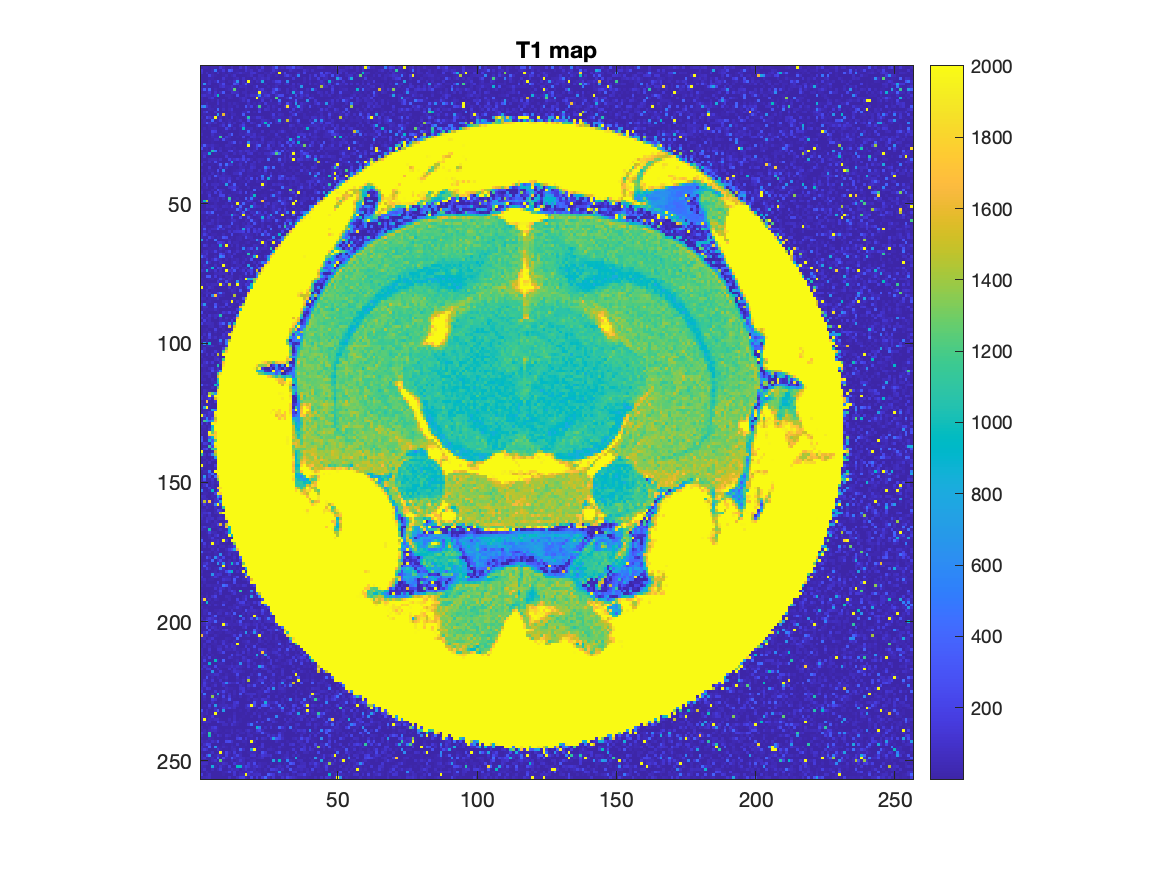
\includegraphics[width=0.3 \linewidth]{figures/T1_map/T1_20month_map.png}
				\\
				\end{array}$
			\caption{$T_1$ Mapping}
		\end{figure}
	\end{frame}

		\begin{frame}
		\frametitle{$T_2$ Mapping}
		\begin{figure}
			$\begin{array}{ccc}
			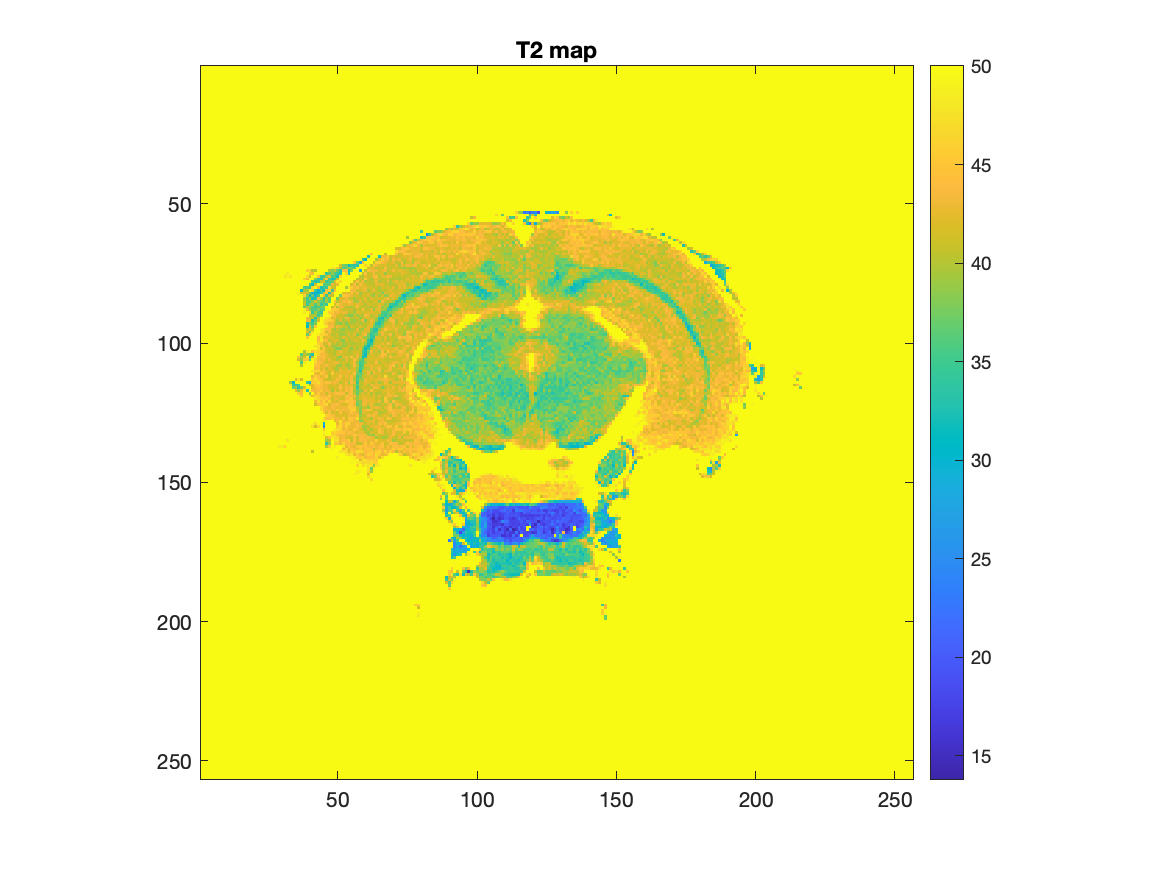
\includegraphics[width=0.3 \linewidth]{figures/T2_map/T2_6week_map.png}
			&
			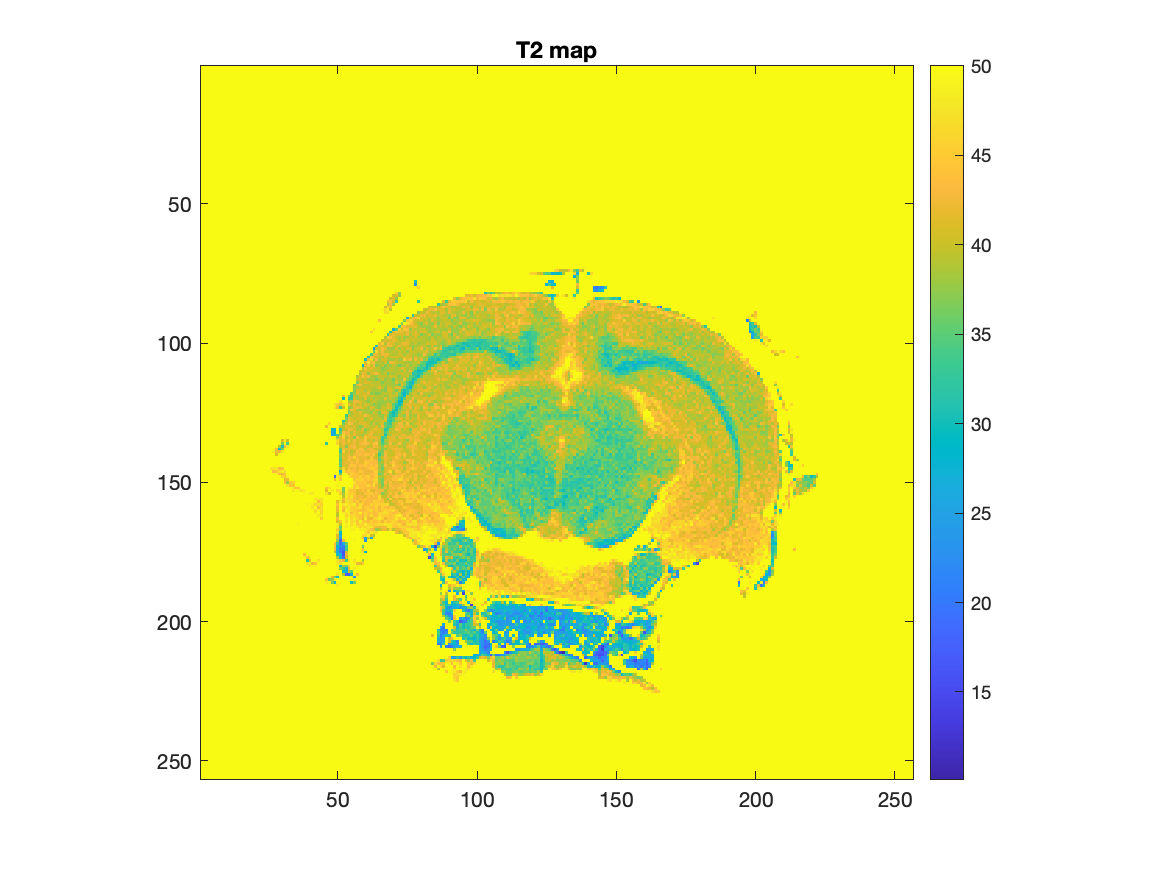
\includegraphics[width=0.3 \linewidth]{figures/T2_map/T2_4month_map.png}
			&
			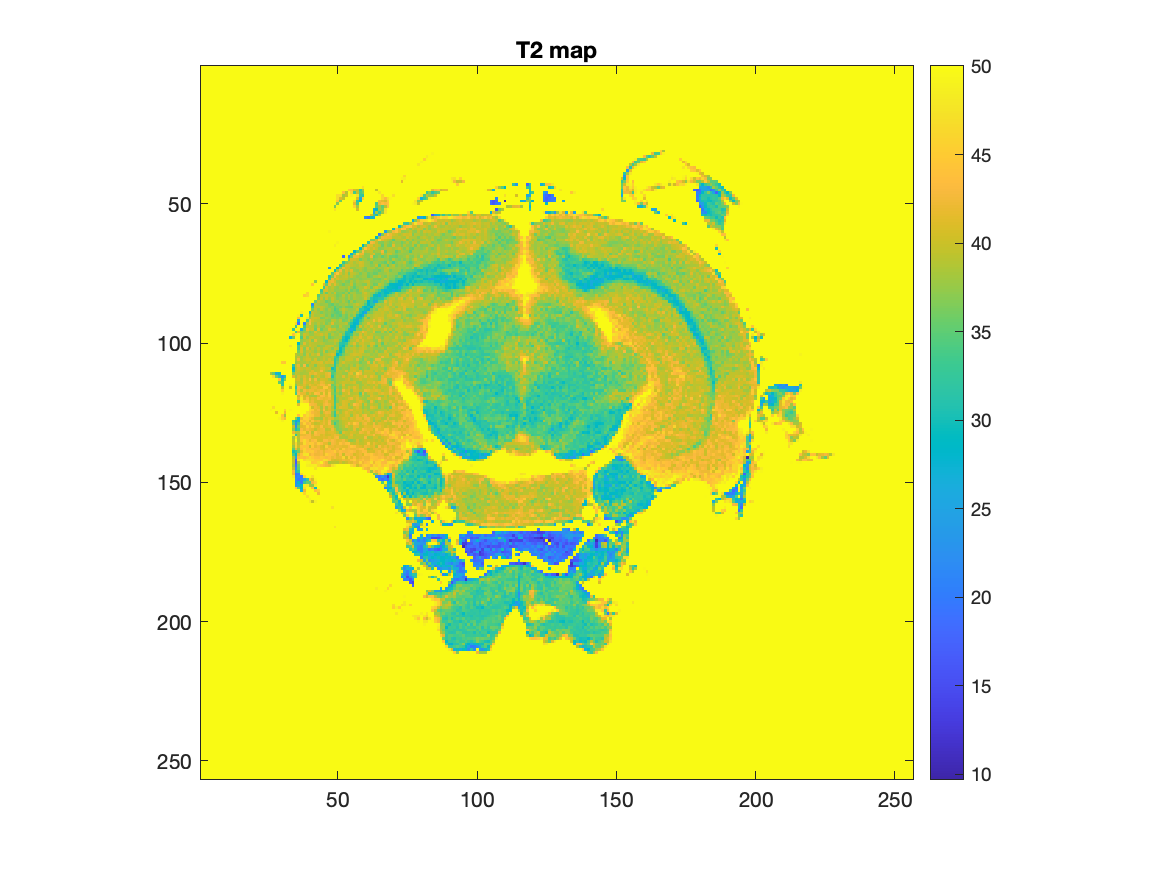
\includegraphics[width=0.3 \linewidth]{figures/T2_map/T2_20month_map.png}
			\\
			\end{array}$
			\caption{$T_2$ Mapping}
		\end{figure}
	\end{frame}
	
	\begin{frame}
		\frametitle{$T_2^*$ Mapping}
		\begin{figure}
			$\begin{array}{ccc}
			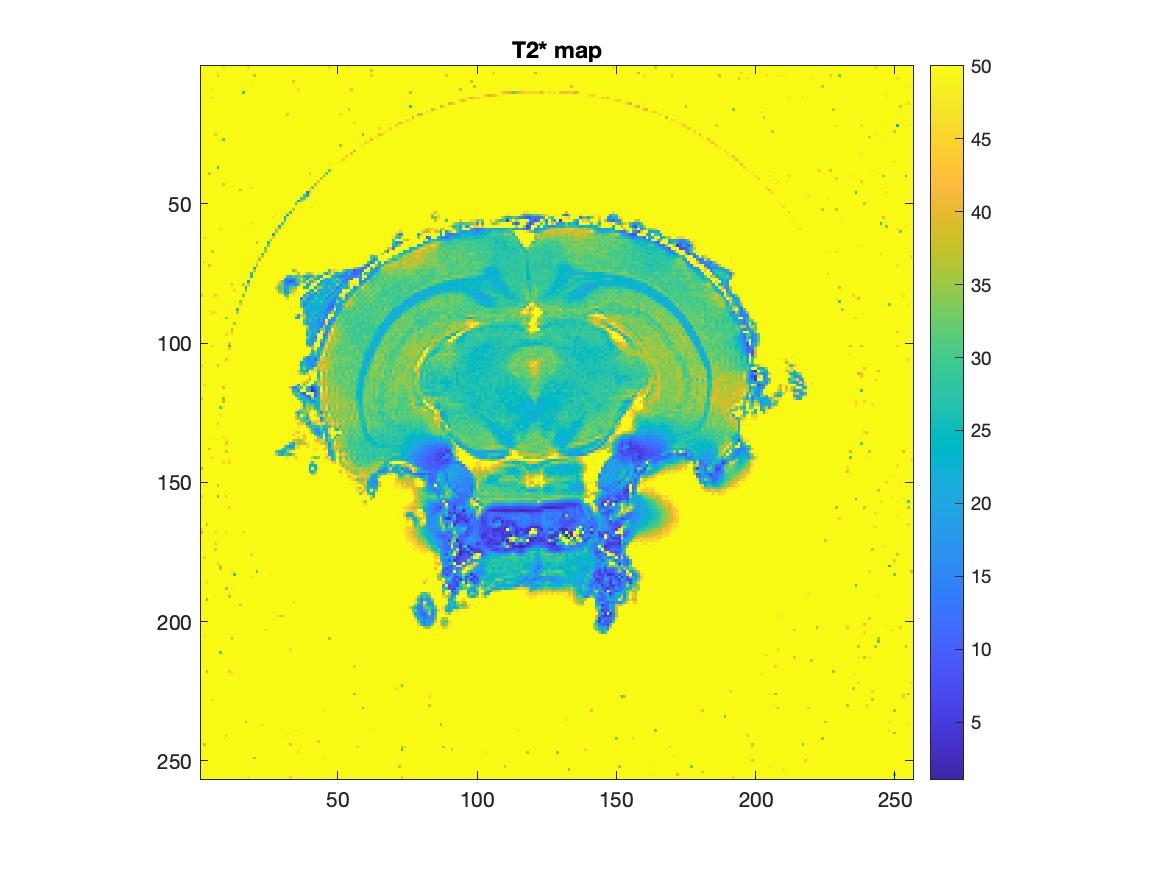
\includegraphics[width=0.3 \linewidth]{figures/T2star_map/T2star_6week_map.png}
			&
			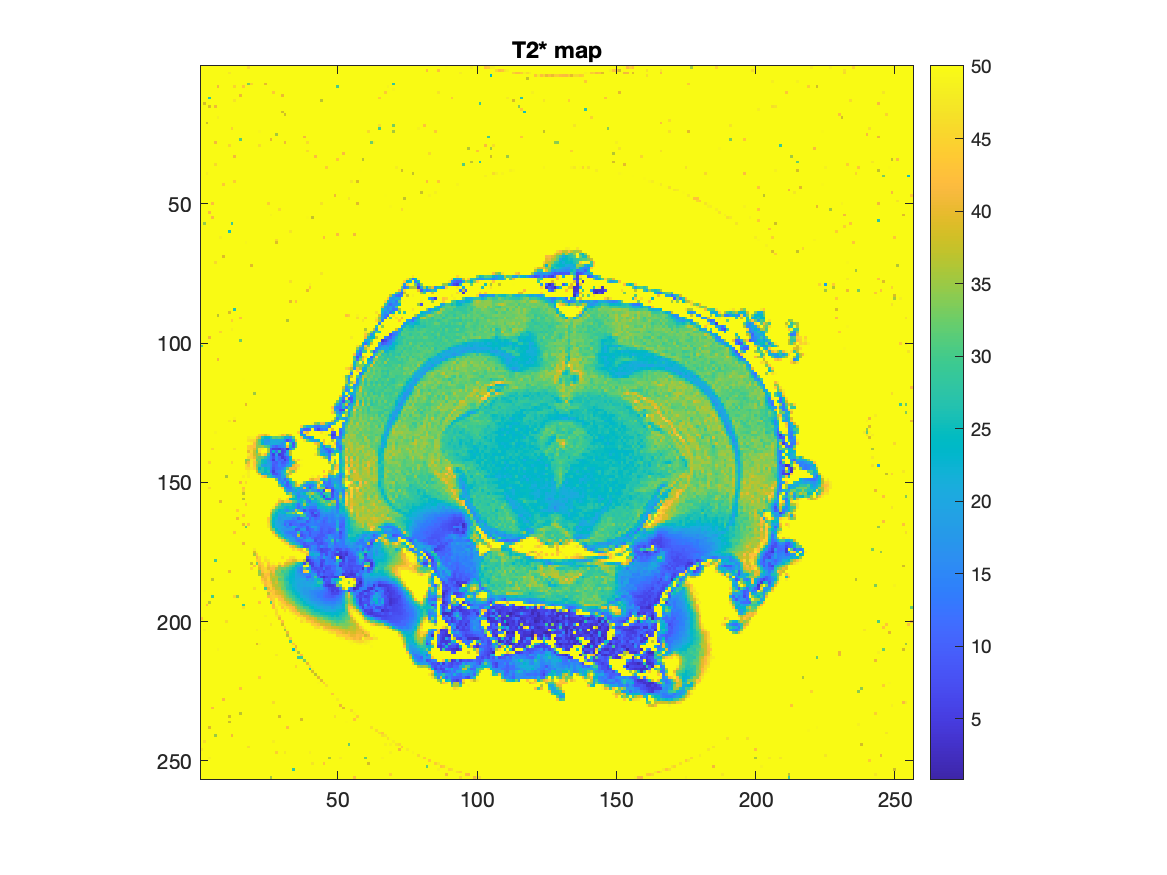
\includegraphics[width=0.3 \linewidth]{figures/T2star_map/T2star_4month_map.png}
			&
			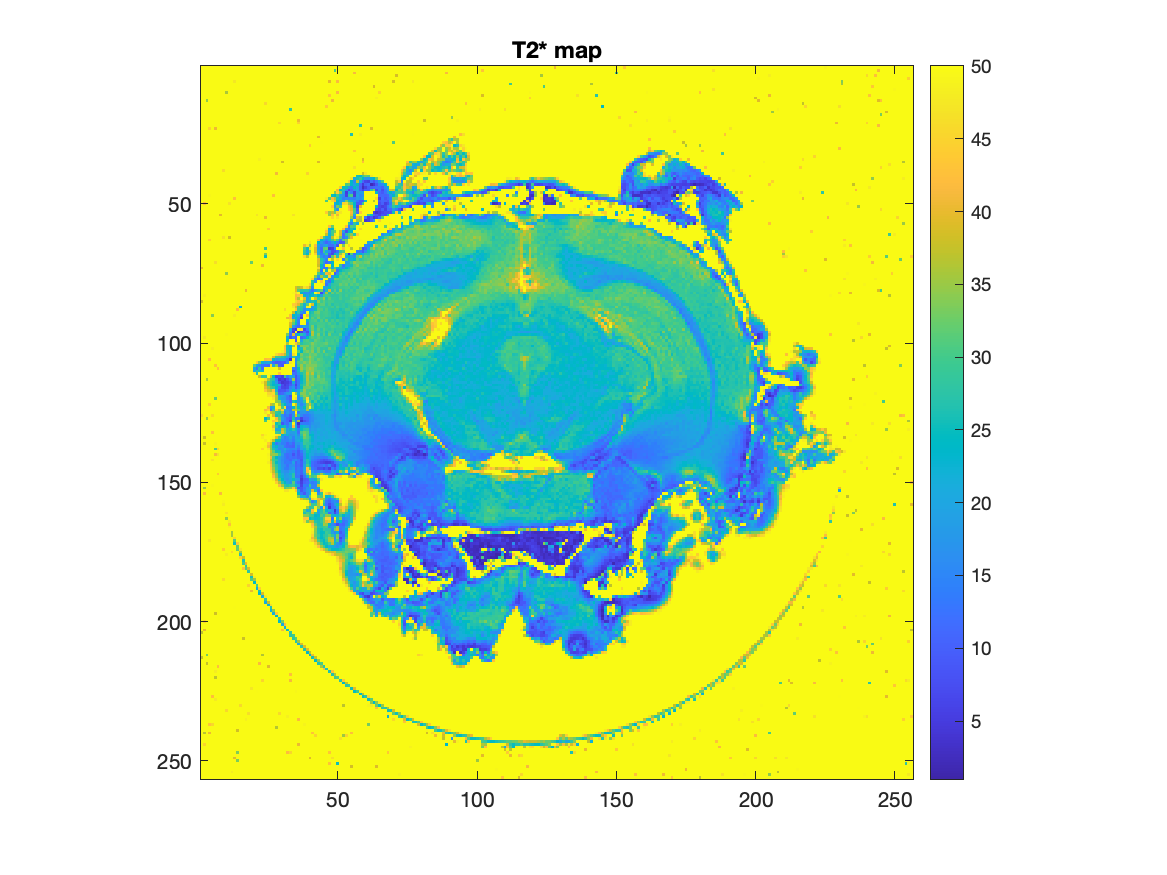
\includegraphics[width=0.3 \linewidth]{figures/T2star_map/T2star_20month_map.png}
			\\
			\end{array}$
			\caption{$T_2^*$ Mapping}
		\end{figure}
	\end{frame}
	
	\section{Discussion}
	
	\begin{frame}[allowframebreaks]
		\frametitle{References}
		\bibliographystyle{apacite}
		\bibliography{reference.bib}
	\end{frame}
\end{document}